\documentclass[../TDE6_rsf.tex]{subfiles}%

\begin{document}
\section[s]"1"{Impédance équivalente}
\iftoggle{student}{ % pour version student
	\iftoggle{corrige}{ % version avec corrigé : affiche juste la correction
		\begin{enumerate}
			\item On commence par convertir le circuit avec les impédances complexes~:
			      \begin{itemize}
				      \item $\Zu_{C_1} = \frac{1}{\jj C_1\w}$~;
				      \item $\Zu_L = \jj L\w$~;
				      \item $\Zu_{C_2} = \frac{1}{\jj C_2\w}$.
			      \end{itemize}
			      On peut ensuite déterminer l'impédance équivalente à l'association en
			      parallèle de $L$ et $C_2$. Avec les admittances, on a
			      \begin{gather*}
				      \Zu\ind{eq,1}
				      = \frac{1}{\frac{1}{\Zu_{C_2}} + \frac{1}{\Zu_L}}
				      = \frac{1}{\jj C_2\w + \frac{1}{\jj L\w}}
				      = \frac{\jj L\w}{1 - \w^2LC_2}
			      \end{gather*}
			      Il suffit alors de faire l'association en série de $\Zu_{C_1}$ et de
			      $\Zu\ind{eq,1}$~:
			      \begin{gather*}
				      \boxed{
					      \Zu\ind{eq} = \frac{1}{\jj C_1\w} + \frac{\jj L\w}{1 - \w^2LC_2}}
			      \end{gather*}
			      Il n'est ici pas nécessaire d'aller plus loin dans le calcul.

			\item Ici, on utilise que $\Zu_R = R$ et comme précédemment, on effectue
			      l'association en parallèle des $R$ et $C$ de droite avant de faire
			      l'association en série de $R$ et $C$ de gauche avec cette impédance
			      équivalente~:
			      \begin{gather*}
				      \Zu\ind{eq, 1}
				      = \frac{1}{\frac{1}{\Zu_1} + \frac{1}{\Zu_C}}
				      = \frac{1}{\frac{1}{R} + \jj C\w}
				      = \frac{R}{1 + \jrcw}
			      \end{gather*}
			      Et on a donc finalement
			      \begin{gather*}
				      \boxed{
					      \Zu\ind{eq} = R + \frac{1}{\jj C\w} + \frac{R}{1 + \jrcw}}
			      \end{gather*}
		\end{enumerate}
	}{ % énoncé
		Déterminer l'impédance complexe équivalente de chacun des dipôles ci-dessous
		en RSF.
		\begin{center}
			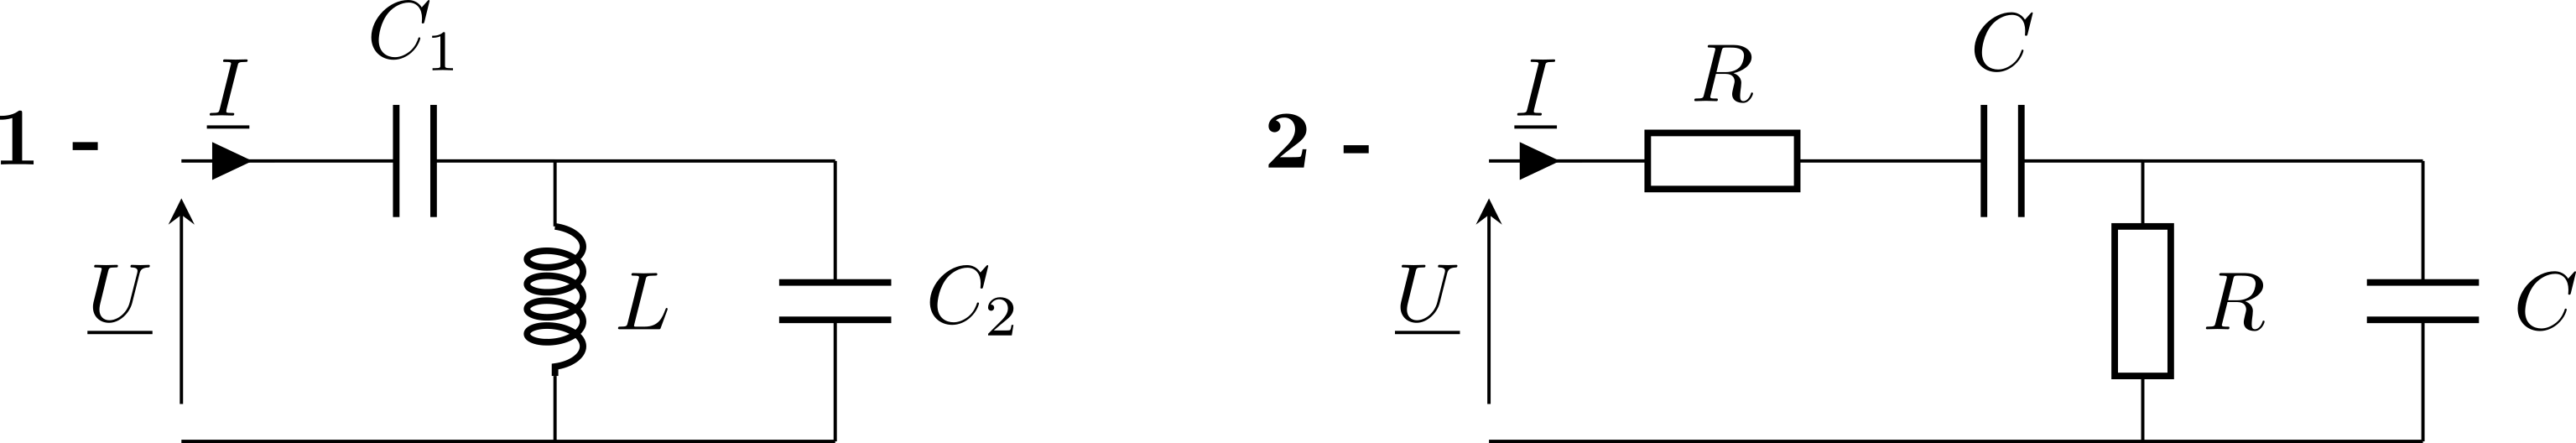
\includegraphics[width=.8\linewidth]{exo1_plain}
		\end{center}
	}%
}{% pour version prof
	\iftoggle{corrige}{% pour version avec corrigé : question ET réponse
		Déterminer l'impédance complexe équivalente de chacun des dipôles ci-dessous
		en RSF.
		\begin{center}
			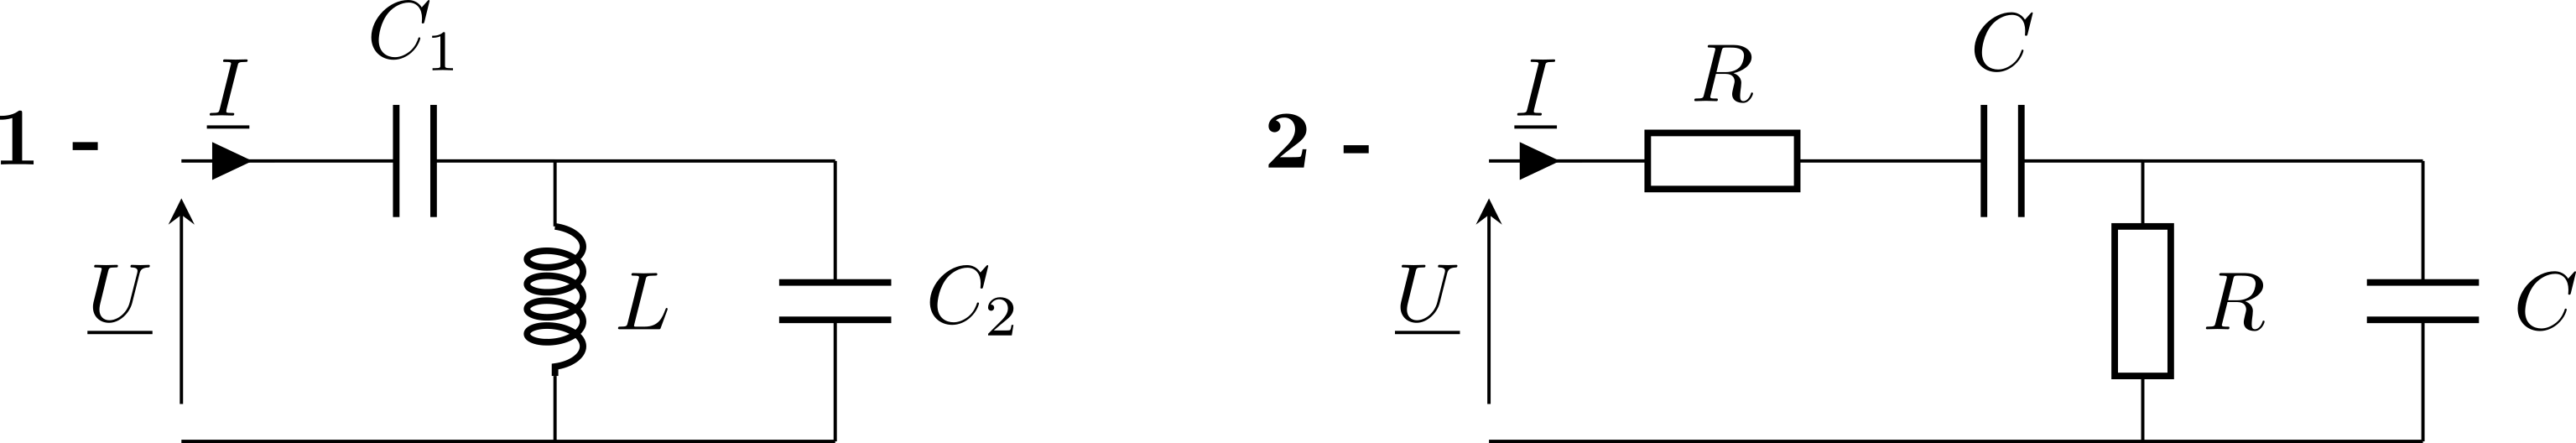
\includegraphics[width=.8\linewidth]{exo1_plain}
		\end{center}
		\begin{answ}%
			\begin{enumerate}
				\item On commence par convertir le circuit avec les impédances complexes~:
				      \begin{itemize}
					      \item $\Zu_{C_1} = \frac{1}{\jj C_1\w}$~;
					      \item $\Zu_L = \jj L\w$~;
					      \item $\Zu_{C_2} = \frac{1}{\jj C_2\w}$.
				      \end{itemize}
				      On peut ensuite déterminer l'impédance équivalente à l'association
				      en parallèle de $L$ et $C_2$. Avec les admittances, on a
				      \begin{gather*}
					      \Zu\ind{eq,1}
					      = \frac{1}{\frac{1}{\Zu_{C_2}} + \frac{1}{\Zu_L}}
					      = \frac{1}{\jj C_2\w + \frac{1}{\jj L\w}}
					      = \frac{\jj L\w}{1 - \w^2LC_2}
				      \end{gather*}
				      Il suffit alors de faire l'association en série de $\Zu_{C_1}$
				      et de $\Zu\ind{eq,1}$~:
				      \begin{gather*}
					      \boxed{
						      \Zu\ind{eq} = \frac{1}{\jj C_1\w} + \frac{\jj L\w}{1 - \w^2LC_2}}
				      \end{gather*}
				      Il n'est ici pas nécessaire d'aller plus loin dans le calcul.

				\item Ici, on utilise que $\Zu_R = R$ et comme précédemment, on effectue
				      l'association en parallèle des $R$ et $C$ de droite avant de faire
				      l'association en série de $R$ et $C$ de gauche avec cette impédance
				      équivalente~:
				      \begin{gather*}
					      \Zu\ind{eq, 1}
					      = \frac{1}{\frac{1}{\Zu_1} + \frac{1}{\Zu_C}}
					      = \frac{1}{\frac{1}{R} + \jj C\w}
					      = \frac{R}{1 + \jrcw}
				      \end{gather*}
				      Et on a donc finalement
				      \begin{gather*}
					      \boxed{
						      \Zu\ind{eq} = R + \frac{1}{\jj C\w} + \frac{R}{1 + \jrcw}}
				      \end{gather*}
			\end{enumerate}
		\end{answ}%
	}{ % énoncé uniquement
		Déterminer l'impédance complexe équivalente de chacun des dipôles ci-dessous
		en RSF.
		\begin{center}
			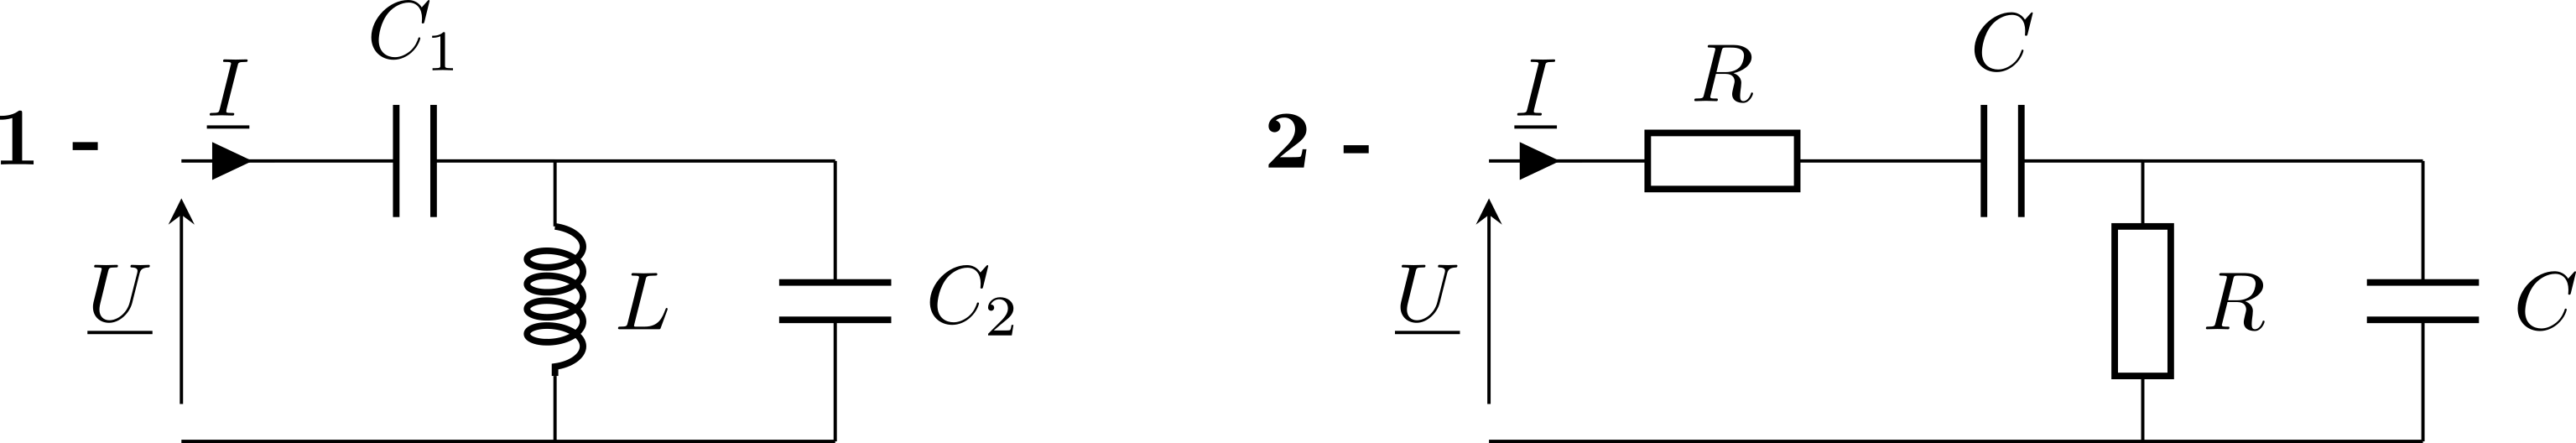
\includegraphics[width=.8\linewidth]{exo1_plain}
		\end{center}
	}
}

\end{document}
